%***************************************************************************
\section{Propagation of the Prior Uncertainties}\label{sec:reflood_prior_uq}
%***************************************************************************

% Opening paragraph
The quantified prior uncertainties of the input parameters are propagated through the \gls[hyper=false]{trace} model of \gls[hyper=false]{feba} to assess (and verify) the prior level of prediction uncertainties.
Independent samples are generated from the prior \glspl[hyper=false]{pdf} of the $27$ selected input parameters (Tables~\ref{tab:trace_model_parameter_1}-\ref{tab:trace_model_parameter_2})
and the \gls[hyper=false]{trace} model of \gls[hyper=false]{feba} is run using the sampled parameters values.

% Explaining the figure
Figs.~\ref{fig:ch2_plot_base_case_216_tc}, \ref{fig:ch2_plot_base_case_216_dp}, and~\ref{fig:ch2_plot_base_case_216_co} show the nominal \gls[hyper=false]{trace} predictions (i.e., the prediction with the nominal values of the input parameters) in comparison with the experimental data for \gls[hyper=false]{feba} test No. $216$ for three selected outputs of different types:
the clad temperature $TC$ at the mid-height assembly, the pressure drop $DP$ of the middle axial segment, and the liquid carryover $CO$ (up to the saturation of the collecting tank at $10\,[kg]$), respectively.
\bigtriplefigure[pos=tbhp,
                 mainlabel={fig:ch2_plot_base_case_216},
			           maincaption={Nominal \gls[hyper=false]{trace} predictions (thick lines) for \gls[hyper=false]{feba} test No. $216$ in comparison with the experimental data (crosses) for three selected outputs. The thin lines in each panel indicate the predictions from $50$ selected realizations of the uncertainty propagation of the input parameters.},
			           mainshortcaption={Nominal \gls[hyper=false]{trace} predictions for \gls[hyper=false]{feba} test No. $216$ in comparison with the experimental data for three selected outputs.},%
			           leftopt={width=0.31\textwidth},
			           leftlabel={fig:ch2_plot_base_case_216_tc},
			           leftcaption={Mid-height clad temperature ($TC$)},
			           midopt={width=0.31\textwidth},
			           midlabel={fig:ch2_plot_base_case_216_dp},
			           midcaption={Mid. pressure drop ($DP$)},
			           rightopt={width=0.31\textwidth},
			           rightlabel={fig:ch2_plot_base_case_216_co},
			           rightcaption={Liquid carryover ($CO$)},
			           spacing={},
			           spacingtwo={}]
{../figures/chapter2/figures/plotBaseCase216TC}
{../figures/chapter2/figures/plotBaseCase216DP}
{../figures/chapter2/figures/plotBaseCase216CO}

% Comments on how the base looks like
The comparison between the nominal \gls[hyper=false]{trace} predictions and the corresponding experimental data for the clad temperature and the pressure drop are satisfactory.
\gls[hyper=false]{trace} seems to capture all the important features of the transient in \gls[hyper=false]{feba} test No. $216$.
That is, \gls[hyper=false]{trace} predicts well the behavior of the reflood curve during the transient; while for the $DP$ output \gls[hyper=false]{trace} predicts well the behavior of channel flooding.
Note that in Fig.~\ref{fig:ch2_plot_base_case_216_dp} the transient between the two equilibrium values indicates the flooding of the channel between axial level $1.7$ and $2.3\,[m]$ from an initial pure steam flow (low pressure drop) to mixture (rising) and eventually a pure liquid flow (higher pressure drop). 
Note also that Fig.~\ref{fig:ch2_plot_base_case_216_tc} is the prediction at the axial level $1.9\,[m]$, a level within the axial segments of the pressure drop.
On the other hand, there is a strong apparent bias (over-prediction) of the \gls[hyper=false]{trace} predictions with respect to the liquid carryover.

% Make observation about variation in time and amplitude
The thin lines plotted in each panel of Fig.~\ref{fig:ch2_plot_base_case_216} indicate the predictions from $50$ selected realizations of the uncertainty propagation.
Particularly with respect to the clad temperature output, the predictions exhibit large variations both in terms of amplitude (vertical) and phase (horizontal).
Specifically for the latter, the timing of important events like the time of quenching varies significantly across realizations.
Moreover, for all the three outputs shown in the figure, the experimental data seems to be within the parametrization of \gls[hyper=false]{trace} according to the assumed prior uncertainties for the parameters.

\begin{sidewaysfigure}
	\centering
	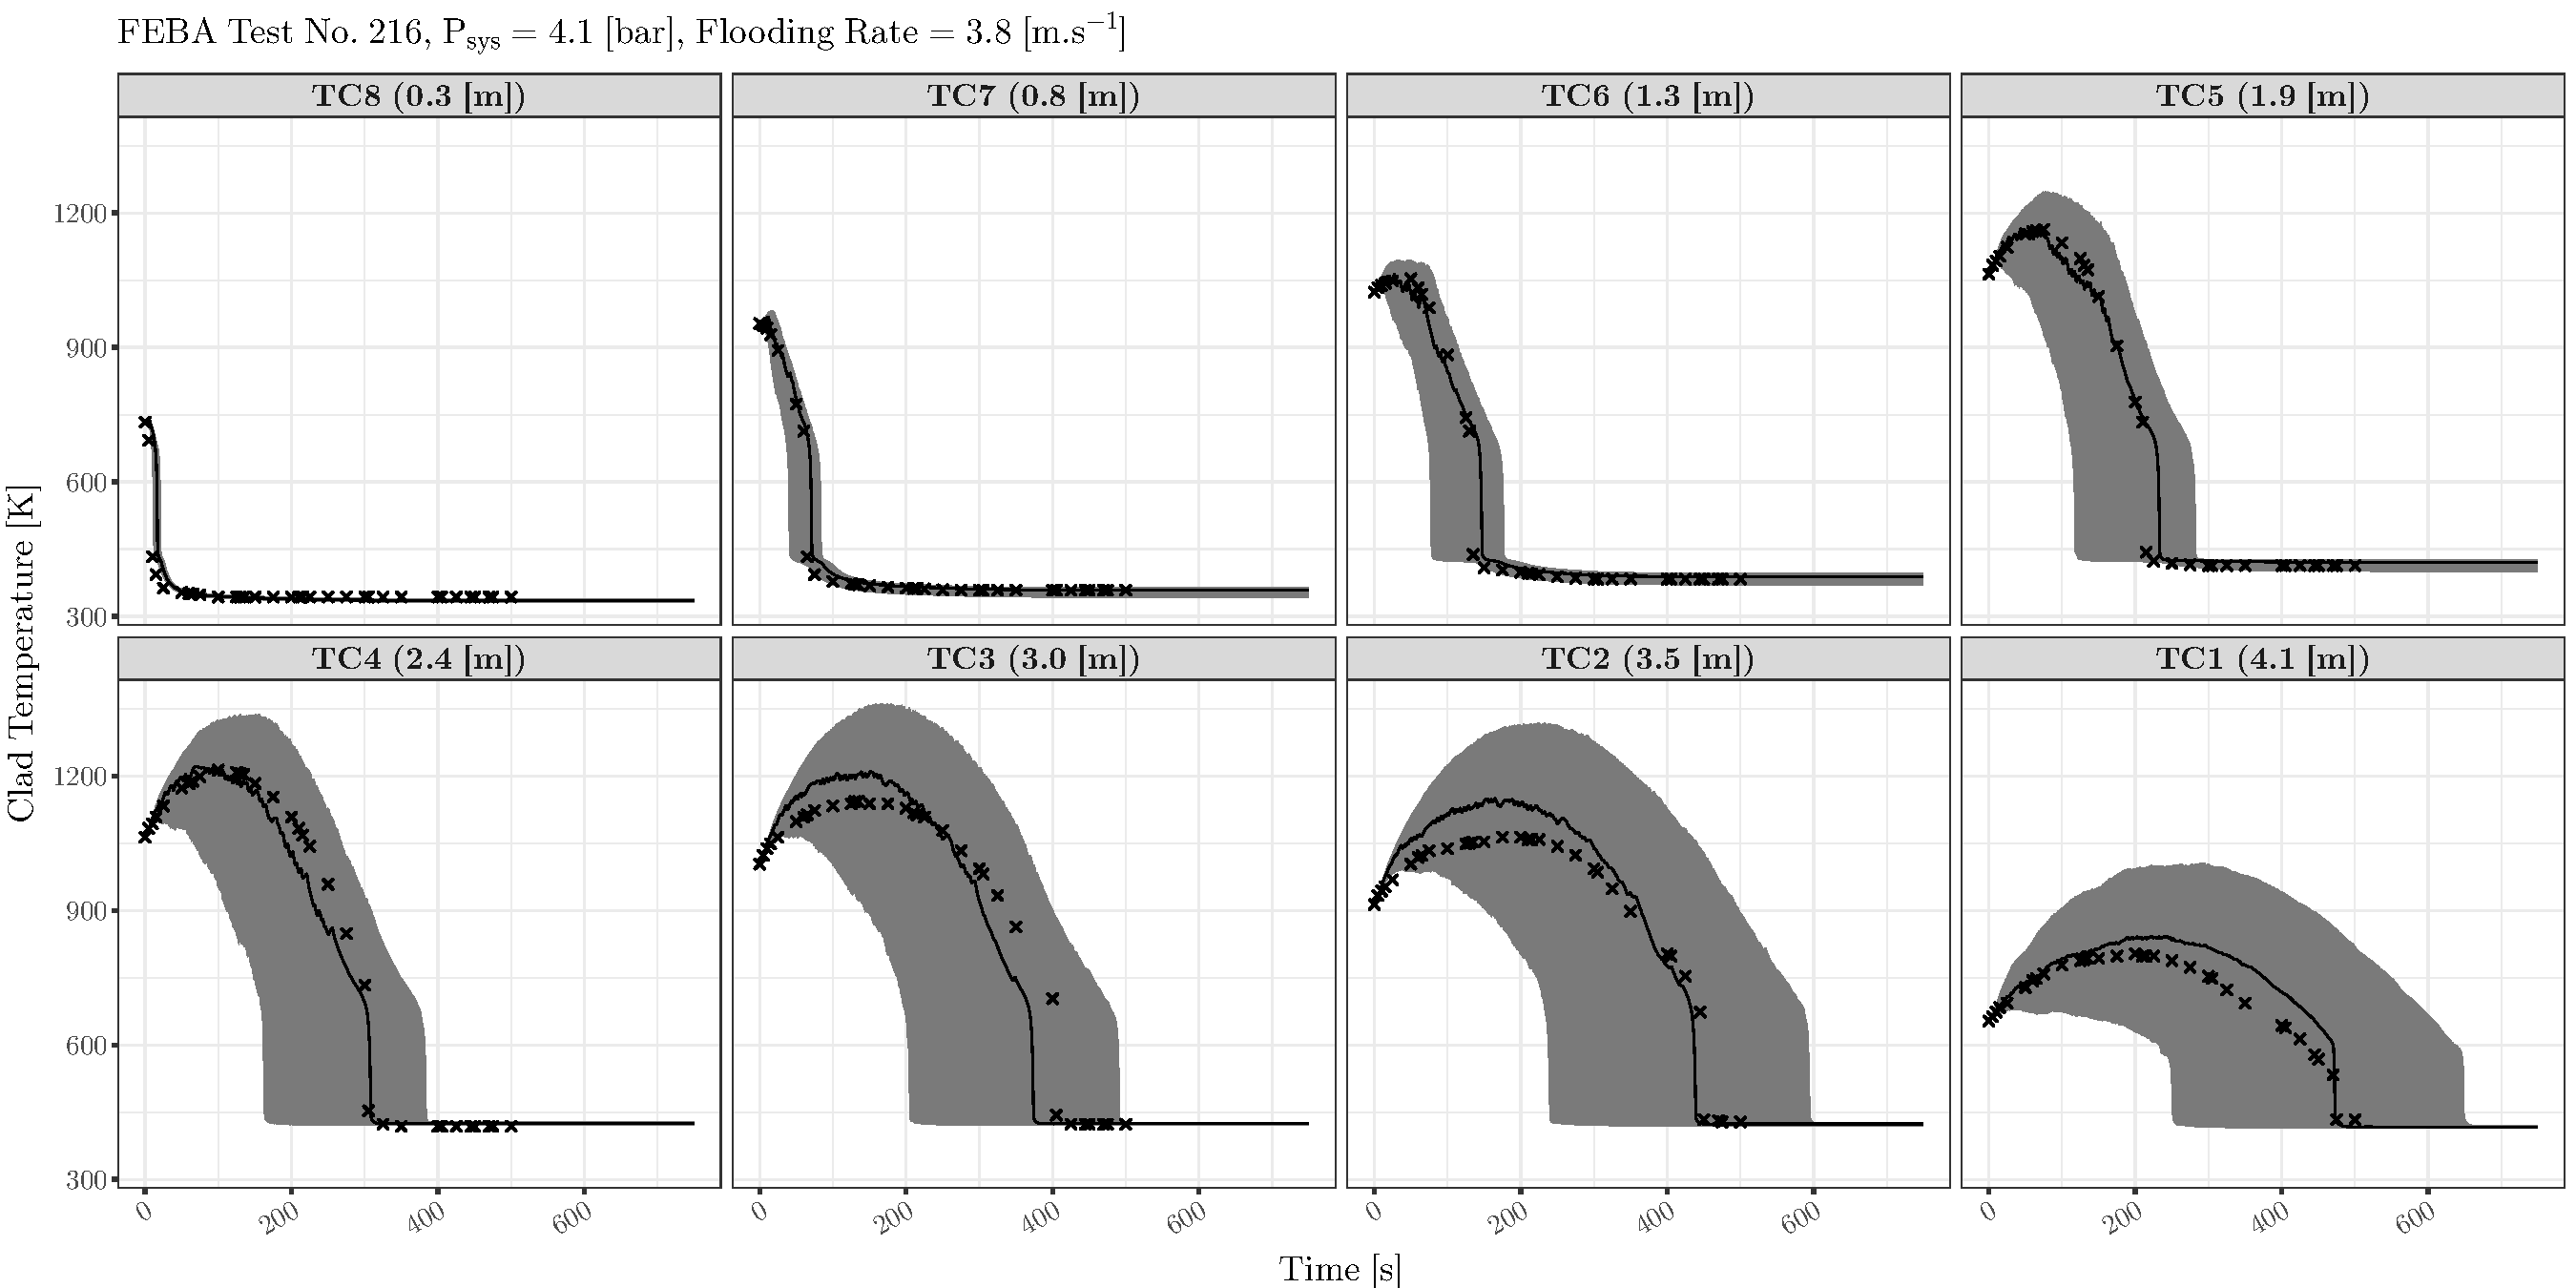
\includegraphics[width=0.90\textwidth]{../figures/chapter2/figures/plotTraceUQPriorTC216}
		\captionof{figure}[Propagation of the $27$ input parameters prior uncertainties on FEBA test No. $216$ for the clad temperature output ($TC$).]{Propagation of the $27$ input parameters prior uncertainties on FEBA test No. $216$ for the clad temperature output ($TC$). The uncertainty bounds correspond to the symmetric ($95\%$) probability; solid lines and crosses indicate the simulation with the nominal parameters values and the experimental data, respectively.}
	\label{fig:ch2_plot_trace_uq_prior_tc_216}
\end{sidewaysfigure}

Figs.~\ref{fig:ch2_plot_trace_uq_prior_tc_216}, \ref{fig:ch2_plot_trace_uq_prior_dp_216}, and~\ref{fig:ch2_plot_trace_uq_prior_co_216} show the complete results of the uncertainty propagation for the three types of output for \gls[hyper=false]{feba} test No. $216$ based on $1'000$ samples of input parameters values.
The prediction uncertainty bands plotted in each panel of the figures refer to the pointwise symmetric $95\%$ probability.
That is, they are constructed based on the intervals between the $2.5$-th and $97.5$-th percentiles of each output type at each time step.
Similar plots showing the results of all the $6$ \gls[hyper=false]{feba} tests are given in Appendix~\ref{app:tbl_results_uq_feba}.

% FEBA Test No. 216 Prior Uncertainty Propagation, TC
Fig.~\ref{fig:ch2_plot_trace_uq_prior_tc_216} shows the uncertainty propagation results for the clad temperature $TC$ output at all eight axial levels.
As observed, for each axial level, the experimental data is well enveloped within the wide prediction uncertainty bands. 
The uncertainty band becomes wider starting from the start of the transient up to the time of quenching.
Furthermore, the uncertainty bands also become wider for the $TC$ predictions moving from the bottom to the top of the assembly.
Lastly, as observed, the nominal \gls[hyper=false]{trace} predictions tends to have larger discrepancy with the experimental data above the mid-height assembly.
Although the time of quenching at all axial levels are well predicted, the $TC$ predictions above the mid-height assembly are underestimated during the transient up to the time of quenching. 
% FEBA Test No. 216 Prior Uncertainty Propagation, DP
\bigfigure[pos=H,
           opt={width=1.0\textwidth},
           label={fig:ch2_plot_trace_uq_prior_dp_216},
           shortcaption={Propagation of the $27$ input parameters prior uncertainties on FEBA test No. $216$ for the pressure drop output ($DP$).}]
{../figures/chapter2/figures/plotTraceUQPriorDP216}
{Propagation of the $27$ input parameters prior uncertainties on FEBA test No. $216$ for the pressure drop output ($DP$). The uncertainty bound corresponds to the symmetric ($95\%$) probability; solid lines and crosses indicate the simulation with the nominal parameters values and the experimental data, respectively.}

Fig.~\ref{fig:ch2_plot_trace_uq_prior_dp_216} shows the uncertainty propagation results for the pressure drop $DP$ output at all four axial segments.
The plots in the figure shows the same pointwise symmetric $95\%$ probability of the prediction uncertainty as before.
As observed, there is no major discrepancy between the \gls[hyper=false]{trace} predictions and the experimental data and the uncertainty bands cover the experimental data well, especially during the transient (i.e., the ramp between two equilibrium values).

% FEBA Test No. 216 Prior Uncertainty Propagation, CO
Finally, Fig.~\ref{fig:ch2_plot_trace_uq_prior_dp_216} shows the uncertainty propagation results for the liquid carryover $CO$ output.
As mentioned, although there is a large discrepancy between the nominal \gls[hyper=false]{trace} prediction and the experimental data, the prediction uncertainty covers the experimental data.
In particular, the propagation of the prior input parameters uncertainties results in large band that is skewed toward the lower values of the predictions uncertainties. 
\begin{figure}[!h]
    \centering
    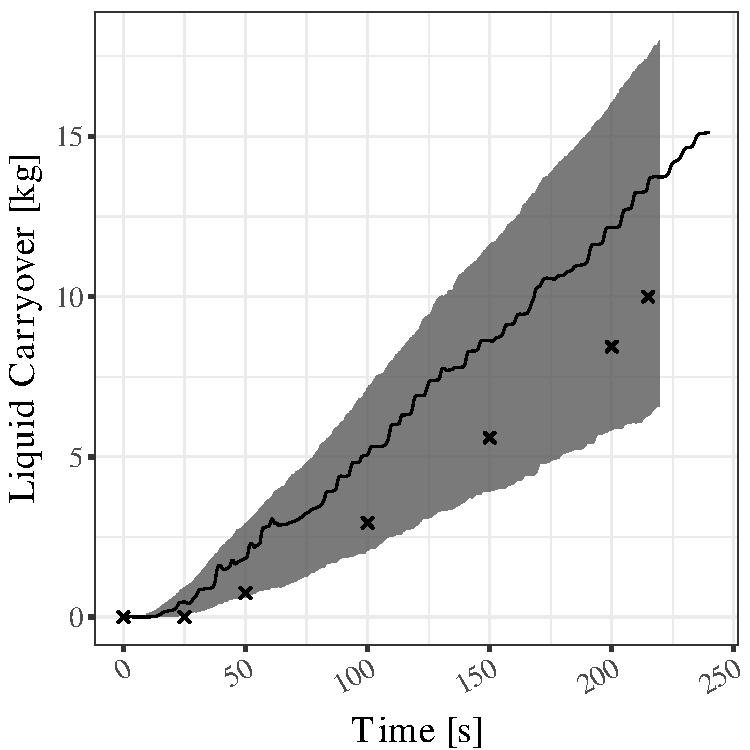
\includegraphics[width=0.5\textwidth]{../figures/chapter2/figures/plotTraceUQPriorCO216}
    \caption[Propagation of the $27$ input parameters prior uncertainties on FEBA test No. $216$ for the liquid carryover output ($CO$).]{Propagation of the $27$ input parameters prior uncertainties on FEBA test No. $216$ for the liquid carryover output ($CO$). The bound corresponds to the symmetric ($95\%$) probability; solid lines and crosses indicate the simulation with the nominal parameters values and the experimental data, respectively.}
    \label{fig:ch2_plot_trace_uq_prior_co_216}
\end{figure}
